\chapter{Assessment of Instrumentation Performance }
%\\ \color{green} POST PUBLIC REVIEW VERSION\color{black}}
\label{ch:performanceassessment}
{\color{magenta}{Contributing author: COM, AK }}{\color{blue}{ -- needs attention  }}

\noindent
\begin{tcolorbox}
\parbox{\textwidth}{
\emph{\textbf{Key Points}
\begin{itemize}
    \item All performance evaluations of potential or currently used instrumentation
    \item B...
    \item C...
    \item D...
\end{itemize}
}}
\end{tcolorbox}


The quality of measured data that is supposed to be used in real-time applications is of immense importance. Modern technologies to assimilate measured data into forecasting models usually have automatic algorithms that blacklist data that is out of range or in other ways suspicious, because bad data is often worse for the forecast model than no data. 

While low quality data can be compensated with longer collection periods or in general longer time-series for non real-time applications such as plant assessment and configuration, resource assessment, etc\., this is not possible in real-time environments, where the data has to be quality checked at the time of retrieval and processed or dismissed. 

Quality control and clear assessment criteria are therefore important tools for the success of the application using real-time measurements. 

In this chapter, we will describe challenges and mitigation strategies for the measurement data processing and quality control. 



\section{Measurement Data Processing {\color{blue}{needs attention}}}\label{sec:dataqa}



\subsection{Known issues of nacelle wind speeds and mitigation methods}

From a theoretical perspective, it can be expected that wake effects from the rotating blades are strongest at high speeds and low speeds that affect the mean wind flow, but not so much the correlation in the "normal" operating range. When plotting nacelle anemometer measured data in a scatter plot, where the linear relationship is strong in the range 3-12m/s and along the linear part of the power curve, this becomes most apparent. Below cut-in and above the wind speed where the power curve gets flat, the linear relationship does not hold any more. It has also been shown with frequency distributions that met mast anemometers produce an approximate Weibull distribution, where nacelle mounted instruments often produce strong biases at the lower wind speeds affected by wake effects.

This is due to 2 effect:
\begin{enumerate}
    \item wake effects from rotating blades
    \item Yaw misalignment of wind turbine
\end{enumerate}

In order to make use of nacelle mounted instrumentation corrections are necessary. The problems associated with these known issues are described in the following together with possible correction methodologies. 

\subsubsection{Wake effects from rotating blades}
Drechsel et al. [2012] found out that the wake effects of nacelle measured wind speeds are highest up until the cut-in wind speed and above approximately 10m/s, where the power curve starts getting flat.
Allik et al. [2014] found out in a study with nacelle mounted cup anemometers, nacelle mounted sonic anemometers and a reference met mast that the mean of the three measurements did not coincide very well. The nacelle wind speed measurements, due to the wake effects of the blades, have a much lower mean. The correlations however were strong between cup anemometer and met mast anemometer and even stronger between sonic anemometer and met mast readings within the range of 3-12m/s. 

Jing et al. \cite{Jing2020} also found that blade wakes affect the measurement of nacelle anemometer, result in the inconsistency between nacelle wind speed (NWS) and free stream wind speed, which seriously affects the power forecasting and performance evaluation of wind turbine.



\subsubsection{Yaw misalignment of wind turbine}

Held et al. \cite{Held2019} reports that due to the limitation of line-of-sight measurements and the limited number of focus positions of a scanning Lidar, assumptions are necessary to derive useful inflow characteristics at the turbine nacelle. The horizontally homogeneous inflow assumption is violated, if a wake impinges the field of view of one of the Lidar beams. In such situations, the turbine yaw misalignment measurements show large biases which require the detection and correction of these observations.



\subsection{Application of nacelle wind speeds in Real-time NWP Data Assimilation} \label{subsec:nacelle_wind_speeds_in_nwp_data_assimilation}

The only recorded project to date that carried out dedicated real-time studies with nacelle wind speeds in a real-time forecasting environment so far is the US Department of Energy funded “Wind Forecasting Improvement Project” (WFIP). The project had a demonstration phase of 1-year and used 410 nacelle wind speeds for the data assimilation of NOAAs models [Wilzcak, 2014, Marquis, 2014]. 

One of the main findings in the experiment was that the nacelle wind speeds were contaminated too much by wake effects to be useful as individual measurements. Due to the constraints in the data assimilation techniques, it was important to find a strategy that made it possible to use the raw data from the cup anemometers. The research team of NOAA found that the best way to handle the contaminated data was to average the individual turbine data per wind farm and then blacklist those measurements that were outside the range of 2 standard deviations from the mean of the wind farm. This is a reasonable constraint to ensure that measurements contaminated by wake effects will not be passed into the assimilation program. 

Additionally, the measurements were averaged over the nearest model grid point in the numerical weather prediction model. By doing this, it was possible to remove systematic biases and make use of the direct outcome of the model at the grid points. 

To summarise, the strategy to use all 411 nacelle measured wind speeds at 23 wind farms has been: 

\begin{itemize}
    \item averaging wind speed measurements over each wind farm
    \item blacklisting measurements that were more than two times a STD from the mean
    \item interpolating and averaging at the nearest grid point of the NWP model
    \item BIAS correcting at the model grid points
\end{itemize}


The advantage of this approach is that wake effects are smoothed out through the averaging within the wind farm and averaging at the NWP model grid points ensures that bias corrections are brought forward to the model result, i.e. the wind power forecast. In this way, it could be demonstrated that nacelle wind speeds can become useful signals seen from a general forecasting perspective.  


Pinson and Hagedorn \cite{PinsonHagedorn2012} used a different path to reduce uncertainty of the 633 meteorological stations with cup anemometers that they compared to model results. Their assumption was made according to the recorded uncertainty of unbiased state of the art anemometer uncertainty, which is a standard deviation of around 0.5m/s. It was shown that this was a reasonable and valid assumption. However, it is not known how much this assumption is dependent on the number of measurement units and their distribution. Therefore, such assumptions must be considered with care. 



\section{Uncertainty of instrumentation Signals }\label{sec:instrumentuncertainty}

In section \ref{} it was described that requesting uncertainty measures from instrumentation in real-time is unrealistic, but that a standing data value that is determined at the setup/calibration of the instrument and provided as part of the standing data, might be feasible.
{\color{blue}{comment SW 210715: This first sentence should be changed! I believe we must provide some uncertainty even with the live data. I think real time data is provided with uncertainty in many cases, It is difficult but can be done. }}
In that way, the instrument specific uncertainty could be accounted for in the handling of measurements. 

\textbf{Alternative instrumentation signal uncertainty estimations}
One alternative is to carry out an uncertainty estimation with e.g. the Monte-Carlo method described in \cite{jcgm2011} (pp23-33). 

Another alternative is to add a mean uncertainty value to raw measurements, as applied by Pinson and Hagedorn \cite{PinsonHagedorn2012} in an experiment over Ireland and Denmark with wind measurements from standard met masts [Pinson and Hagedorn, 2012 p7]. 

If a more standardised technical requirement is desirable, the JCGM guides \cite{jcgm2008,jcgm2008a,jcgm2009, jcgm2011,jcgm2012} offer a valuable general source, also applied in meteorology and oceanography. In that way, a harmonisation of "best practices" with these directly related real-time disciplines can be achieved. In fact, the guides do not only consider the measurand as a physical quantity, but also provide guidance to the conceptual design and the theoretical analysis of measurements and methods. 


%\section{Uncertainty of Measurements}\label{sec:measurementuncertainty}
%{\color{blue}{Comment from SW (25.06.2021:I think we can remove this section. as there is already a section on uncert. of signals.}}

\section{Quality control of measurements for real-time use}\label{sec:quality_control}

{\color{blue}{Author: COM -- needs more authors/discussion}}




{\color{blue}{Comment from COM (27.06.2021:
In Meteorology (see e.g. \cite{Lucio2018,Lucio2018a}:
(1) data management errors:
    - data transcription and collection
    - errors that occurred during data manipulation (e.g. duplication of data sequences)
    - standardization of practices (e.g. measurement units, reference times) 
    
(2) measurement errors: 
    - temporal or spatial consistency in the data
    - errors produced at the moment of sampling as a result of :
        - instrumental malfunction
        - calibration
        - exposure problems

---------------------------------------------------------

\textbf{Comments from COM: 19.08.2021}

---------------------------------------------------------

I like EPA's definition of QC and QA and would like to discuss this -- with the goal in mind that we are aiming to provide a practical guideline! \\

The EPA's Meteorological guidance for the use of observational data (see \url{https://www.epa.gov/sites/default/files/2020-10/documents/mmgrma_0.pdf} )says the following:  
Quality Assurance/Quality Control (QA/QC) procedures are required to ensure that the data collected meet standards of reliability and accuracy.\\  

- \textbf{Quality Control (QC)} is defined as those operational procedures that will be routinely followed during the normal operation of the monitoring system to ensure that a measurement process is working properly. These procedures include periodic calibration of the instruments, site inspections, data screening,data validation, and preventive maintenance.  The QC procedures should produce quantitative documentation to support claims of accuracy.  \\

- \textbf{Quality Assurance (QA)} is defined as those procedures that will be performed on a more occasional basis to provide assurance that the measurement process is producing data that meets the data quality objectives (DQO).  These procedures include routine evaluation of how the QC procedures are implemented (system audits) and assessments of instrument performance (performance audits).\\

The QAQC procedures should be documented in a Quality Assurance Project Plan (QAPP) and should include a "sign-off" by the appropriate project or organizational authority. The QAPP should include the following [63]: 

1.  Project description - how meteorology is to be used 

2.  Project organization - how data validity is supported 

3.  QA objective - how QA will document validity claims 

4.  Calibration method and frequency - for meteorology 

5.  Data flow - from samples to archived valid values 

6.  Validation and reporting methods - for meteorology 

7.  Audits - performance and system 

8.  Preventive maintenance 

9.  Procedures to implement QA objectives - details

10.  Management support - corrective action and reports \\

It is important that the person providing the QA be independent of the organization responsible for the collection of the data and the maintenance of the measurement systems. 

Ideally, this person should be employed by an independent company.  There should not be any lines of intimidation available to the operators which might be used to influence the QA audit report and actions.  With identical goals of valid data, the QA person should encourage the operator to use the same methods the QA person uses (presumably these are the most comprehensive methods) when challenging the measurement system during a performance audit. 

\textbf{When this is done, the QA task reduces to spot checks of performance and examination of records thus providing the best data with the best documentation at the least cost.}\\


\textbf{For us this recommendation could look like this:} \\
\textbf{1. Project Description and organisation}\\
...    - how measurements are to be used\\
...    - how measurement signals are collected and stored\\
...    - how data validity is defined and reported\\
...    - QA objective and how QA will document validity claims\\
    
\textbf{2. QA procedure and monitoring} \\
...    - Provision and Monitoring is done by an agent independent of the end-user and the data provider (e.g. forecaster, IT consultant)
...    - Regular data validation and verification \\
...    - Performance monitoring and Reporting\\
...    - Corrective Actions according to Reports\\




}}

The purpose of quality control of measurements is to ensure that data can be used for forecasting 

There are 2 time horizons for the quality control: 
\begin{enumerate}
    \item QC in real-time forecasting at the time of receipt; ``black- and white listing''
    \item QC in historic mode: \\ quality control of a specific time interval of data such as a day, a month or one or more years for resource assessment, performance monitoring, model/forecast training/tuning etc. 
\end{enumerate}
{\color{blue}{comment SW 210715: Why should we define that real time QC is a black and white listing? One could also imagine another category of suspicious data that is used but assuming a higher uncertainty than normal so that it influences the forecasts less. At this point I wouldn't exclude such an option.}}
{\color{green}{comment COM 210726: Agree, but it needs to be specified more here. E.g. that in extreme events, suspicious data often show the real happening. Today, I think this is not practices very much to keep algorithms robust, but we should mention that the optimal use is to include the uncertainty...}}



\section{General data quality control (QC)}
repeated values, values out of range limits, formatting of data file/decoding error, consistency of time stamps/chronologically, time averaging definition, site coordinates, instrumentation identification

\subsection{Accuracy and Resolution Limits}
Table \ref{tab:epa_table} shows the EPA [EPA, 2000, 4.5 Sampling Rates] accuracy recommendation that could be used as guidelines for the energy sector as well. 

\begin{table}[h!]
    \centering
    \begin{tabular}{l l l}
Meteorological	        &   System	                  & Measurement \\
Variable	            &   Accuracy                  &	 Resolution \\ \hline\hline
Wind Speed	            & $\pm{0.2}$ m/s              & 0.1 $m/s$ (horizontal\\
                        & (+ 5\% of observed)         & and vertical)\\
 & & \\
Wind Direction          & $\pm{5}$ degrees	          & 1.0 degree \\
(azimuth and elevation) &                             &  \\		
 & & \\
Ambient Temperature     & $\pm{0.5}^\circ$C	          & 0.1 C \\
 & & \\
Dew Point Temperature	& $\pm{1.5}^\circ$C	          & 0.1 C \\
 & & \\
Precipitation	        & $\pm{10}$ \% of observed    & 0.3 mm \\
                        & or $\pm{0.5}$ mm	          &  \\
 & & \\
Pressure	            & $\pm{3}$ mb (0.3 kPa)	      & 0.5 mb \\ \hline
    \end{tabular}
  \caption{United States Environmental Protection Agency's recommended system accuracies and measurement resolution [EPA, 2000, Table 5-1].}
 \label{tab:epa_table}
\end{table}

\subsubsection{Data Sampling Thresholds}

EPA's guidance [EPA, 2000, 4.5 Sampling Rates] are the sampling of data signals and the recommendations regarding data sampling and averaging. EPA recommends for data communication purposes for example that an average over a specific time interval should never have less than 60 signals .    


\section{Historic Quality Control (QC)} 

\subsection{QC for Wind Applications}

In most cases the QC methodology should be designed for both long-term analysis of e.g\. a year and shorter periods such as weekly, monthly or quarterly examination of observational data signals. There are two targets for the validation and quality control:

\begin{enumerate}
\item To identify the amount of valid data submitted.
\item To produce a comprehensive analysis which will provide the wind farm owner with a description of the root of the detected error(s) in the signals.
\end{enumerate}

Simple approaches will not meet these targets. For a number of reasons cross correlation between e.g\. wind farms or solar parks is not a feasible methodology for the verification of observational data signals as it is too much challenged by irregular distances of the generating unit's locations and would only produce justifiable results, when done over long verification periods.

Depending on the significance of the data issue, the time from when an issue with data signals starts until it is diagnosed and solved is too long, if QA is only carried out once per year.


\subsubsection{Practical Methodology for quality control of wind measurement}

Apart from outages in the submission, the validation process of wind speeds is going to be based on statistics over long time periods. The evidence of an error would have to be very convincing until a case would be opened. The methodology to use for the validation is a combination of consistency checks between:
\begin{itemize}
 \vspace{-0.2cm}\item forecasted wind speed versus measured wind speed
 \vspace{-0.2cm}\item forecasted temperature, wind direction against measured values
 \vspace{-0.2cm}\item forecasted power versus active power checked with SCADA MW
 \vspace{-0.2cm}\item Computed active power from measured wind speed versus actual active power
 \vspace{-0.2cm}\item Comparison against previous years of the same wind farm
 \vspace{-0.2cm}\item Comparison to the average error level for wind farms in the same period
\end{itemize}

\subsubsection{Statistical tests and metrics for the QC process}\label{subsubsec:statistical_tests}

{\color{blue}{Comment from COM (21.08.2021): 
There are different methods to test the quality of measurements. 
}}

\subsubsection{A. QC for Wind applications with Forecast Ranges}\label{subsubsec:hist_qc_forecast_ranges}
One practical solution to test measurement signal quality is to use verification methods similar to the verification of forecast errors with the exception that a forecast or a forecast range is used as the reference, because it is the measurement that needs validation. The forecast has a known accuracy level, which is used to find changes in quality in the measurement signals. 

By validating in different sub periods of the year, it can be shown whether the error pattern has been temporary or on a long-term basis. 

By using a variation of different statistical tests, the data basis is large enough to interpret the data accuracy. The following set of statistical metrics are recommended:

\begin{enumerate}
    \vspace{-0.2cm}\item \textbf{BIAS:}\\
The BIAS in itself should be low, but is no guarantee of correctness of the data, because a BIAS can be low for the incorrect reason
    \vspace{-0.2cm}\item \textbf{MAE:}
MAE and BIAS together show, if the data has an offset. 
\vspace{-0.2cm}\item \textbf{RMSE:}
There are few extreme errors, if the ratio RMSE/MAE exceeds 1.3. 
    \vspace{-0.2cm}\item \textbf{CORRELATION:}\\
The correlation allows for easy detection of constant measurements as well as sign errors. 
    \vspace{-0.2cm}\item \textbf{Frequency distribution:}\\
The frequency distribution from e.g\. a one year data set of 15-min mean values of a wind speed should be a smooth curve with decreasing probability of high wind speeds. A temporary instrument fault will be visible as a skewness of the curve. 
Comparing the frequency distributions of an ensemble mean forecast against measurements is recommended in this case, as a mean smooths outliers in the data set.

Positive and negative phase errors between a forecast and measured data tend to cancel each other out over a long enough period. Therefore, a high similarity between two independent time series of the same physical variable can be expected. 
\end{enumerate}

The formulas of the test metrics can be found in the Appendix \ref{appB:metrics}


\subsubsubsection{Long-term verification of met data signals}
In the study, a long-term verification of the data signals from 4 meteorological variables has been carried out. The variables were 
\begin{enumerate}
    \vspace{-0.2cm}\item wind speed
    \vspace{-0.2cm}\item wind direction
    \vspace{-0.2cm}\item air temperature
    \vspace{-0.2cm}\item air pressure
\end{enumerate}

Figure~\ref{fig:met_cor},~\ref{fig:met_mae} and ~\ref{fig:met_bias}  show examples of results of a historic quality control procedure of data signals in form of CORRELATION, MAE and BIAS for 4 variables over a period of 2 years. Each metric is calculated for one wind farm. The ranking for the quality will always be variable dependent. For example temperature varies slower than wind speed and achieves therefore in general a higher correlation.\\


\begin{figure}[h!]
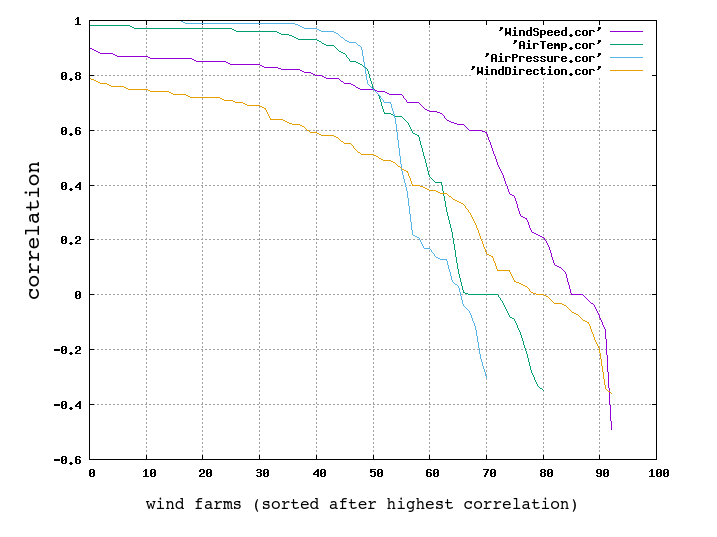
\includegraphics[width=0.75\textwidth]{figures/met_cor.png}
\caption{\textit{Results from a 2 year statistical verification of met data signals on CORRELATION for 4 variables. The x-axis shows wind farms ordered with the highest correlation first.}} 
\label{fig:met_cor}
\end{figure}


\begin{figure}[h!]
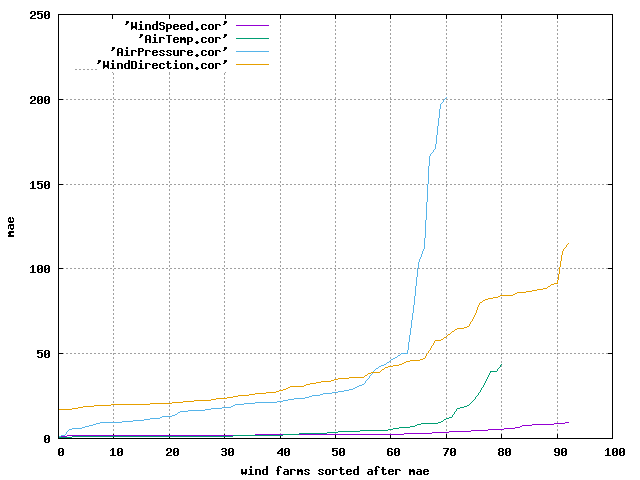
\includegraphics[width=0.7\textwidth]{figures/met_mae.png}
\caption{\textit{Results from a 2 year statistical verification of met data signals measured on MAE for 4 variables. The x-axis shows wind farms ordered with the lowest MAE first. The unit and magnitude is variable dependent and somewhat hides the growth of the wind speed error.}} 
\label{fig:met_mae}
\end{figure}


\begin{figure}[h!]
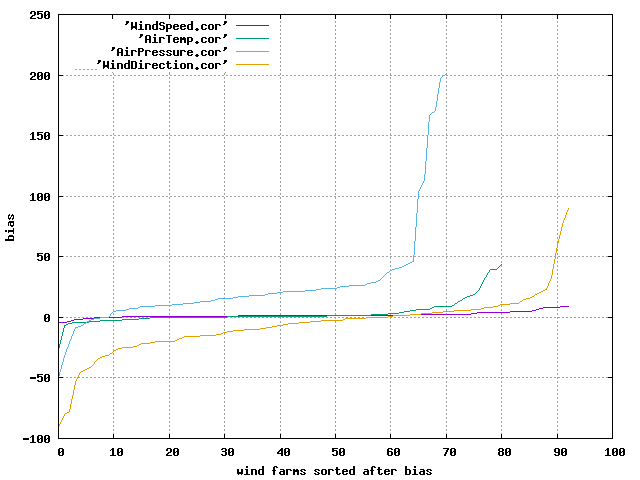
\includegraphics[width=0.7\textwidth]{figures/met_bias.png}
\caption{\textit{Results from a 2 year statistical verification of met data signals measured on BIAS for 4 variables. The x-axis shows wind farms ordered with the lowest BIAS first. The unit and magnitude is variable dependent. Note that the pressure BIAS hides the growth of the wind speed error for the last 30 wind farms.}} 
\label{fig:met_bias}
\end{figure}

With this graphical analysis it is possible to define acceptance limits for the quality of the data in terms of BIAS, MAE and CORRELATION.

\newpage

\subsection{QC for solar applications}

There are several sets of QC tests for historic radiation data (BSRN, SERI QC, QCRad, MESOR, ENDORSE, Journee et al., MDMS (Geuder et al.), ).
The tests in the literature use different limits for individual irradiance components (DHI, GHI, DNI) or parameters derived from these components together with solar position and at times clear sky irradiance. Types of limits are 
\begin{itemize}
    \item physical possible limits
    \item rare limits
    \item extremely rare limits
\end{itemize}
The existing QC tests have been harmonized in the framework of IEA PVPS Task 16 for stations with measurements of all three irradiance components (GHI, DHI, DNI) or two (GHI and DHI or DNI).
The quality control consists of automatic tests and visual inspection by an expert. The  QC results in one flag per time stamp and test. The flag's value is either "data seems ok", "data point was detected as problematic" or "test could not be performed". The latter can occur for a missing time stamp/data or if the test domain was not met and the test could not be applied.\\
The visual inspection of the data is of importance to detect bad data and manually assign the flag. This also includes the control of the meta data (logbook with comments, calibration information). Visual inspection can also help to determine if the time stamps refer to the end of the averaging interval (e.g. 1min, 10min or 1h averaging). The correct interpretation of the timestamps is essential. 
The following tests are defined. All test results are visualized and manual flagging can be used to improve the automatic test results. Some tests are not automated, but purely visual inspections:
\begin{itemize}
    \item   Missing time stamps	
    \item	Missing values	
    \item	K-Tests	
    \item	BSRN Three Component tests	
    \item	extremely rare limits test from BSRN	
    \item	Physically possible limits (PPL) test from BSRN
    \item	Tracker off test
    \item	Visual inspection: Heat map of irradiance with axes hour of the day (y) and day of year	 (x)
    \item	Visual inspection: Shading test: heat map of max irradiance in bins of Sun elevation and azimuth angle	with axes elevation (y) and azimuth (x)
    \item   Visual inspection: deviation of DNI measurement from DNI calculated from GHI and DHI	
    \item	Visual inspection: AM/PM symmetry of the time period	
    \item	Visual inspection: calibration changes by plot of the clear-sky index vs. time	
\end{itemize}



To decide if a data point can be used not only the result of a single flag per timestamp is needed, but all flags for that timestamp and surrounding timestamps must be considered. For the validation of satellite and model derived radiation data the following procedure is recommended. A data point is usable if all individual QC flags are indicating that the data is ok or that the test could not be performed and all measured radiation components are available. Also if 30 percent or more of the timestamps (daytime, solar elevation >0) from one day are flagged, exclude the entire day. Intervals between flagged data that are shorter than 60 min are also excluded. For the determination of the length of the interval only timestamps with elevation >0 are considered. Less stringent exclusion rules could be applied for other purposes, such as the determination of yearly sums.

\subsection{Historic QC other meteorological parameters {\color{red}{Comment from COM (21.08.2021: Do we really need that ? }}}

\section{Real time Quality Control (QC)}



%\subsection{Quality control in historic mode}\label{qa_historic} 
%{\color{green}{Comment from SW (28.06.2021: the text in the subsection "Quality control in historic mode" should be integrated in the subsections above}}
%% this text is now in section \label{subsubsec:qc_forecast_ranges}




%\subsubsection{Challenges and considerations for the QA process{\color{blue}{Author: COM -- needs more authors/discussion}}}\label{subsec:} 

\subsection{Real-time QC for Wind Applications}
{\color{blue}{Comment from COM (23.08.2021: Needs clean up!!! }}

\subsubsection{A. QC for Wind applications with Forecast Ranges}\label{subsubsec:real-time_qc_forecast_ranges}
One practical solution to test measurement signal quality is to use verification methods similar to the verification of forecast errors with the exception that a forecast or a forecast range is used as the reference, because it is the measurement that needs validation. The forecast has a known accuracy level, which is used to find changes in quality in the measurement signals....

\subsubsection{B. QC for Wind applications according to site assessement standards}\lebel{subsubsec:real-time_qc_site-assessment-standard}

For resource or site assessment in the planning phase of a wind farm an IEC standard exists \citep{iec17025-2005E} with an updated version 2 (IEC 61400-12-2:2013), that specifies which tests and what kind of criteria the instrumentation has to fulfil when used for the required tests to be carried out. The IEC 61400-12-2:2013 rules contain the following items:
\begin{itemize}
    \item Extreme winds
    \item Shear of vertical wind profile
    \item Flow inclination
    \item Background turbulence
    \item Wake turbulence
    \item Wind-speed distribution
\end{itemize}

The results of these tests have to be within a pre-defined range to be acceptable. In Appendix F of the 61400-12-1:2005 "Cup anemometer calibration procedure" the calibration of the instruments for measuring wind are specified \cite{iec61400-12-1-2005}.\\


MEASNET (MEASuring NETwork), the "international network for harmonised and recognized measurements in wind energy" has defined so called "Round Robin rules" for calibration of cup anemometers for wind energy \cite{measnet2009}, which are widely used. MEASNET has also  published a number of guidelines regarding instrument calibration and measurement campaigns for the wind industry within the EU project ACCUWIND (\cite{Dahlberg2006,Pedersen2006, Eecen2006}. Lee [2008] found a way of calibrating wind direction sensors with an optical camera.

The Annex D in IEC 61400-12-1:2005 standard states that the "implicit assumption of the method of this standard is that the 10 min mean power yield from a wind turbine is fully explained by the simultaneous 10 min mean wind speed measured at hub height, and the air density" [IEC, 2005, Annex D, Table D.1] and describes the associated measurement uncertainty evaluation principles.  In this respect, the standard refers to the "ISO Guide to the expression of Uncertainty in Measurements" \citep{jcgm2008,jcgm2009,jcgm2012} and its 2 supplements [\citep{jcgm2008a,jcgm2011} from the Joint Committee for Guides in Meteorology (JCGM), where there are two types of measurement uncertainty that are to be accounted for in any standardised measurement taking: 
\begin{enumerate}
    \item systematic errors, which are also known as measurement bias, often associated with offsets of the measured quantity
    \item random errors, which are associated with the fact that 2 measurements of the same quantity are seldom the same
\end{enumerate}

In section 3.1.2 of the guide, \citep{jcgm2008,jcgm2011} it is stated that "the result of a measurement .. is only an approximation or estimate .. of the value of the measurand and thus is complete only when accompanied by a statement of the uncertainty ... of that estimate". Considering this definition, all measurements should ideally have an uncertainty term associated with it. This is impractical in real-time operations, where the value of the measurements lies in the availability of the data at a given time. Therefore, it is unrealistic to request uncertainty measures. However, it could be a standing data value that is determined at the setup of the instrument and provided as part of the standing data. In that way, the instrument specific uncertainty could be accounted for in the handling of measurements.\\ 

The alternative is to carry out an uncertainty estimation with e.g. the Monte-Carlo method described in \citep{jcgm2011} pp23-33) or a mean uncertainty value must be added to raw measurements, as applied by Pinson and Hagedorn in an experiment over Ireland and Denmark with wind measurements from standard met masts [Pinson and Hagedorn, 2012 p7]. If a more standardised technical requirement is desirable, the JCGM guides offer a valuable general source, also applied in meteorology and oceanography. In that way, a harmonisation of "best practices" with these directly related real-time disciplines can be achieved. In fact, the guides do not only consider the measurand as a physical quantity, but also provide guidance to the conceptual design and the theoretical analysis of measurements and methods. 

In the introduction to the Guide [JCGM, 2009], it is stated that “..the principles of this Guide are intended to be applicable to a broad spectrum of measurements”, including those required for:
\begin{itemize}
   \item maintaining quality control and quality assurance in production
   \item complying with and enforcing laws and regulations
   \item calibrating standards and instruments and performing tests throughout a national 
   \item measurement system in order to achieve tractability to national standards developing, maintaining, and comparing international and national physical reference standards, including reference materials 
\end{itemize}

To summarise, the handling and integration of wind power into the electric grid is an equally important step to harness the full potential of the energy resource in an efficient and environmentally friendly way. 


This requires that measurements are trustworthy and maintained to a quality that allows for their use in forecasting tools in order to produce high quality forecasts and thereby reduce the need of reserves. These guides in combination with the IEC 61400-1 standard provide a good foundation for any grid code technical requirement specifications. 

In the following a few specific control procedures for the most common instrumentation are provided.  

\begin{enumerate}
    \item Cup anemometer on a met mast:\\

The accuracy of a single value from a cup anemometer is not high without a 10min time average. The purpose of the 10min averaging process is to eliminate the impact of the turbulent motion, which is generated as a result of frictional forces from the terrain on the air as well as the imbalance in the diurnal cycle and the temperature difference between the air and the surface.
From a 15 minute data delivery of a noise contaminated signal, it is almost impossible to prove the correctness or falsify the data  signals, because some of the values are realistic and others are not.

In contrast to the nacelle measurements, a single cup anemometer on a mast can be inspected at a much lower cost, today even with a drone. Several anemometers can be mounted on the mast and it is at least possible to submit the data directly without giving the wind farm software the possibility to delay, block or manipulate the data.

    \item Cup anemometer on a wind turbine nacelle:\\
      {\color{blue}{Author: COM -- needs more authors/discussion}}
    \item Remote sensing devices:\\
{\color{blue}{Author: COM -- needs more authors/discussion}}




    \item Blade-pressure computed nacelle wind:\\
{\color{blue}{Author: COM -- needs more authors/discussion -- there are areas, where this is used to a great extend and the results are astonishing good as a fit for the produced power. These methods are mainly used for wind farm control; nevertheless they have some important and interesting aspect also for real-time forecasting....}}


\end{enumerate}



\subsection{Real time  QC for solar Forecasting Applications}

For the real-time QC of solar radiation data, the QC methods for historic data can only be partly applied. QC methods requiring visual inspection cannot be applied automatically. Such methods can be used to analyse errors that are detected differently. QC results indicating that the result is suspicious such as the above described tests for rare limits or some versions of the three component tests might lead to too many data gaps, depending on the real-time application. If this is the case, these strict QCs should be adapted with less strict limits or used only for the further analysis of the data once another QC test was not passed. The limits should be defined based on the required data quality and data availability. A site dependence of these limits should be considered. For different instrument options different limits might be required, as e.g. cosine errors of pyranometers vary strongly between different models. Currently no standardised QC for real-time radiation data exist. 



\section{Real time QC other meteorological parameters {\color{red}{Comment from COM (21.07.2021: Do we really need that ? }}}





